\documentclass[xcolor=dvipsnames]{beamer}
\usepackage[T1]{fontenc}
\usepackage[utf8]{inputenc}
\usepackage[english,slovak]{babel}

\usepackage{amsmath}
\usepackage{amsthm}
\usetheme{Pittsburgh}
\useoutertheme{shadow}

\usepackage{graphicx}
\usepackage{caption}
\usepackage{subcaption}


\usepackage{listings}
\lstloadlanguages{Ruby}
\lstset{%
basicstyle=\ttfamily\color{black},
commentstyle = \ttfamily\color{red},
keywordstyle=\ttfamily\color{blue},
stringstyle=\color{orange}}



%-------------------------------------------------------------------------------------
\title{\bf Klasifikácia žiadanej hodnoty Kohonenovou neurónovou sieťou}
\author{Michal CHOVANEC \\Fakulta riadenia a informatiky}

\date[EURP]{\it Júl 2015}
\begin{document}

\begin{frame}
\titlepage
\end{frame}

%-------------------------------------------------------------------------------------
\begin{frame}{\bf Cieľ}

Ako stanoviť žiadanú hodnotu pre robota sledujúceho čiaru?

\begin{figure}[ht]
\begin{center}
\begin{minipage}{0.6\linewidth}
\begin{center}
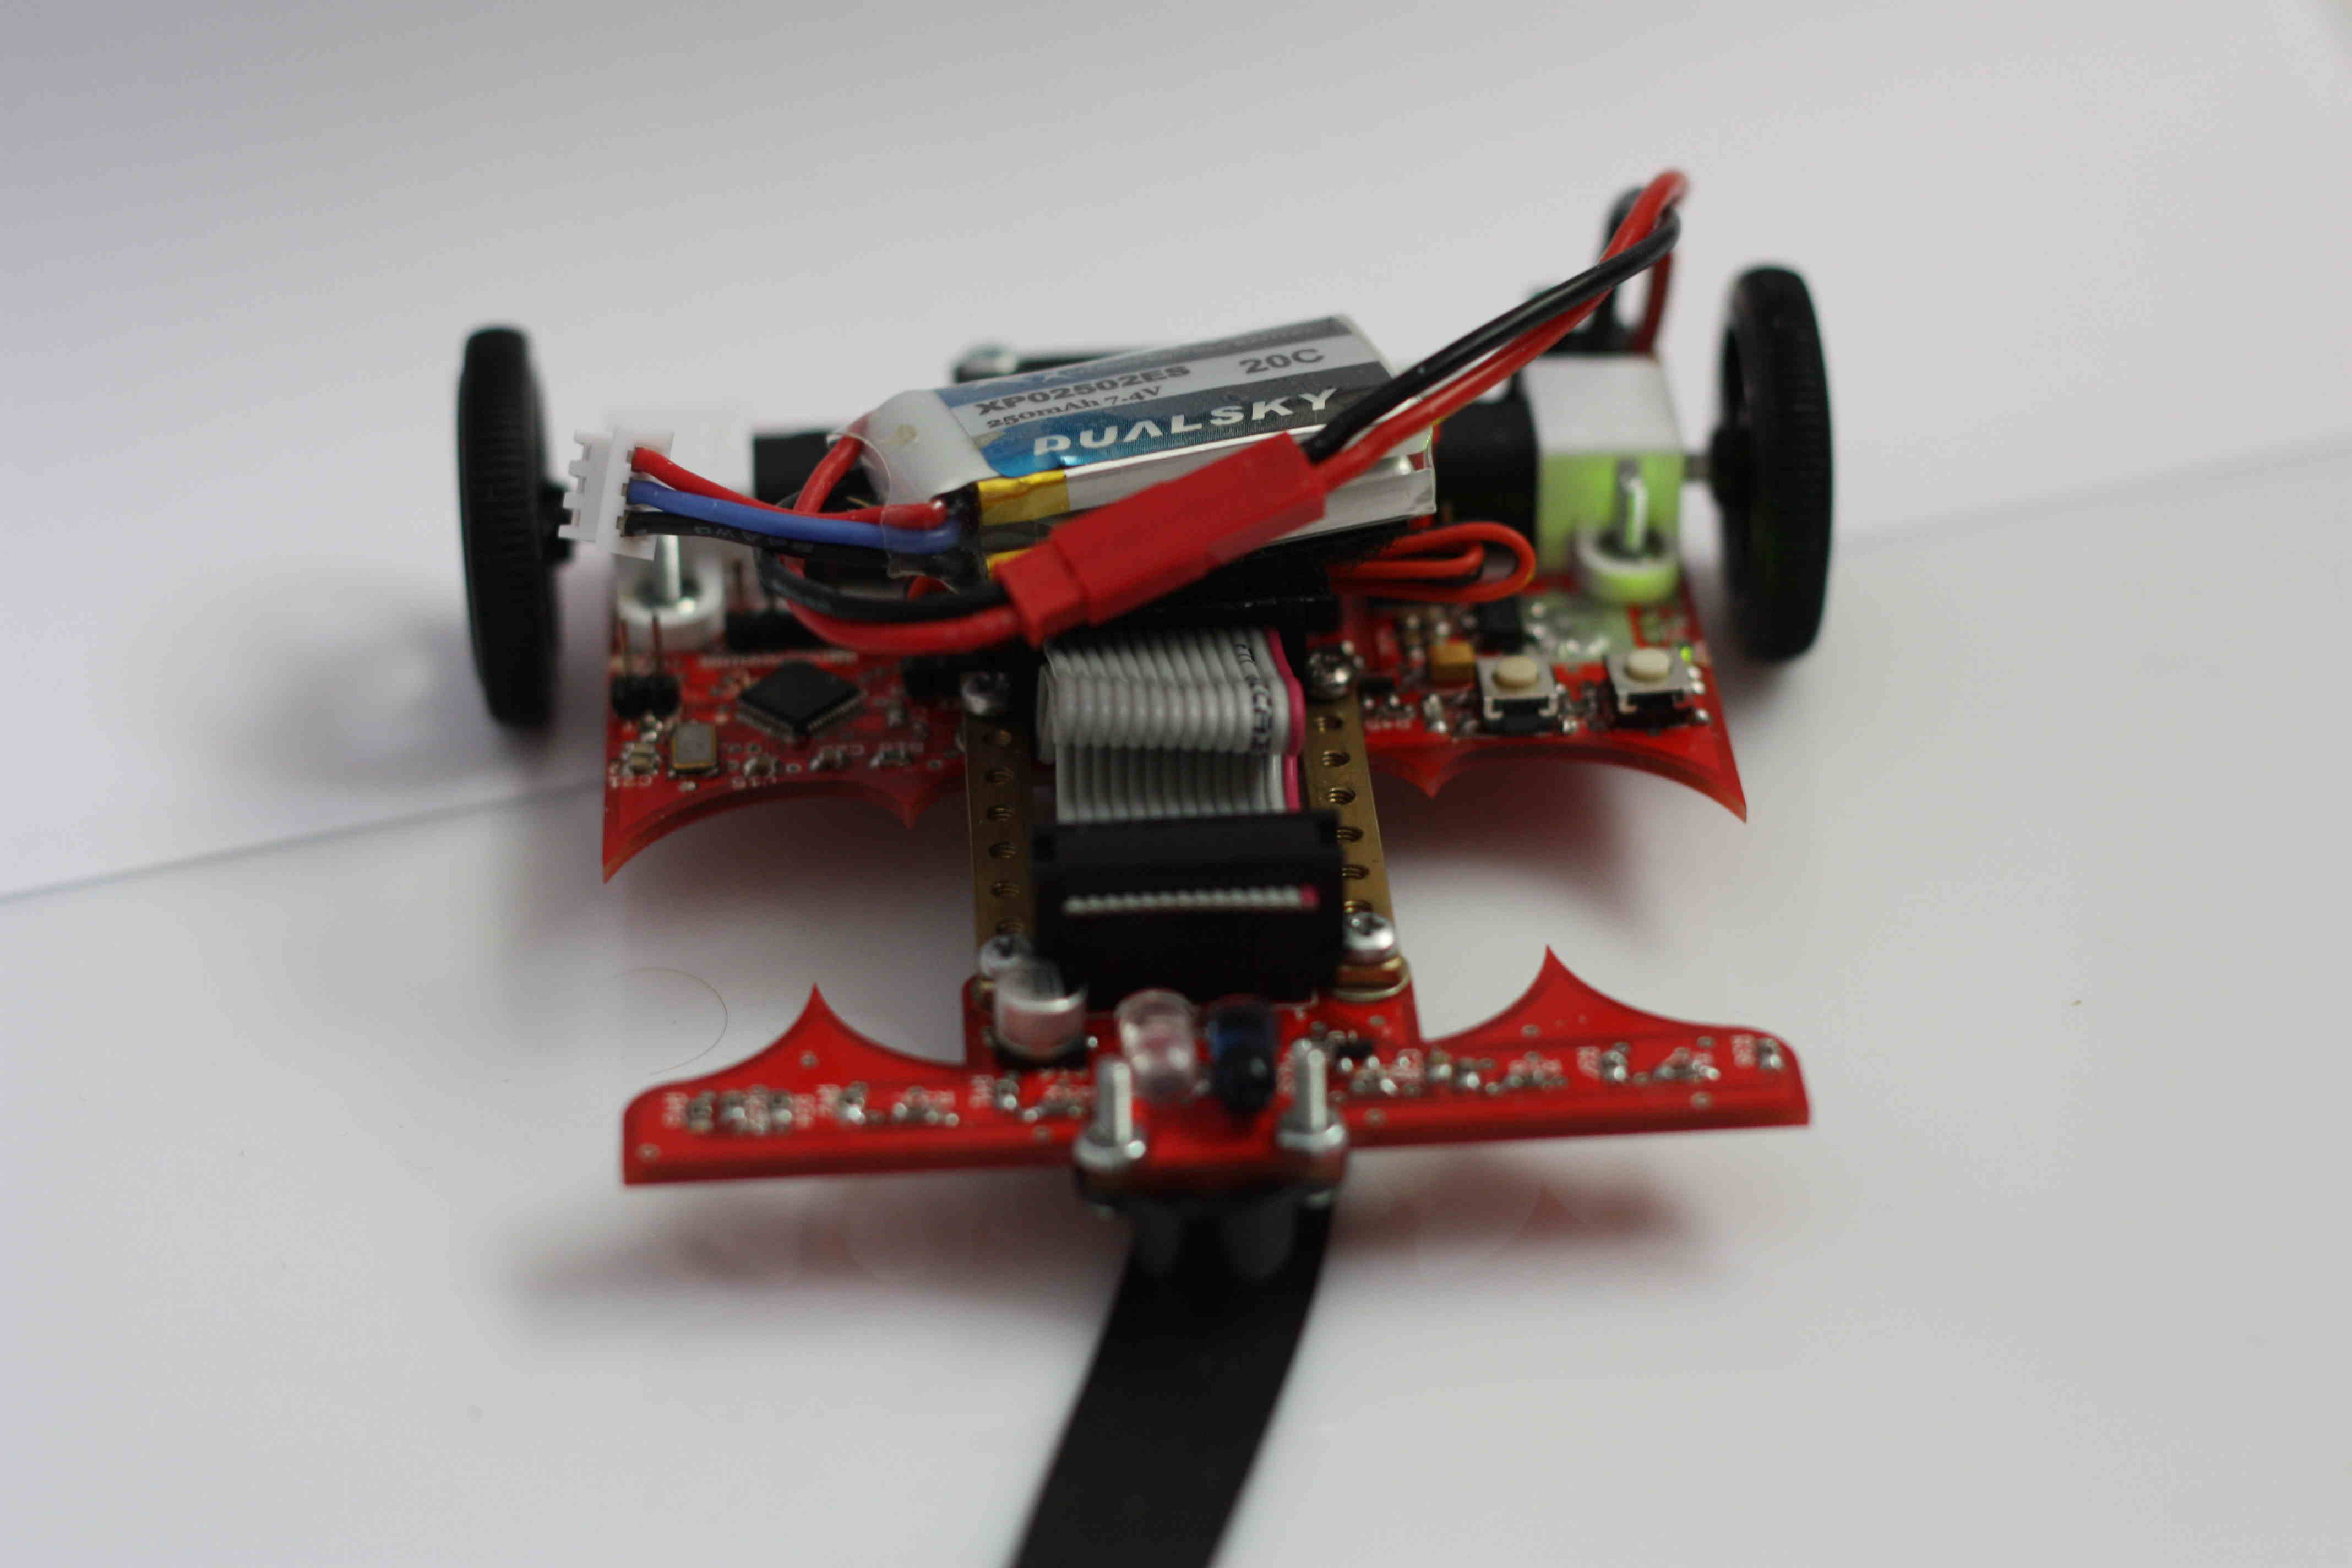
\includegraphics[width=1.0\textwidth]{images/motoko_aftermath_front.jpg}
\end{center}
\end{minipage}
\end{center}
\end{figure}

\end{frame}

%-------------------------------------------------------------------------------------
\begin{frame}{\bf Cieľ}

Riadia sa ,,rýchlosti'' motorov $r(n)$ a $l(n)$.

\begin{align}
\label{eq_basic_robot}
 r(n) &= v(n) - d(n) \nonumber \\
 l(n) &= v(n) + d(n) \nonumber \\
\end{align}

kde \\
$v(n)$ je spoločná ,,rýchlosť'' oboch motorov, \\
$d(n)$ je rozdielová ,,rýchlosť'' motorov. \\
Viera : pre každú zákrutu existujú také  $v(n)$ a $d(n)$, pre ktoré je
$v(n)$ maximálne a poloha čiary $s(n) \approx 0$.

\end{frame}

%-------------------------------------------------------------------------------------
\begin{frame}{\bf Štruktúra regulátora}

\begin{figure}[ht]
\begin{center}
\begin{minipage}{0.8\linewidth}
\begin{center}
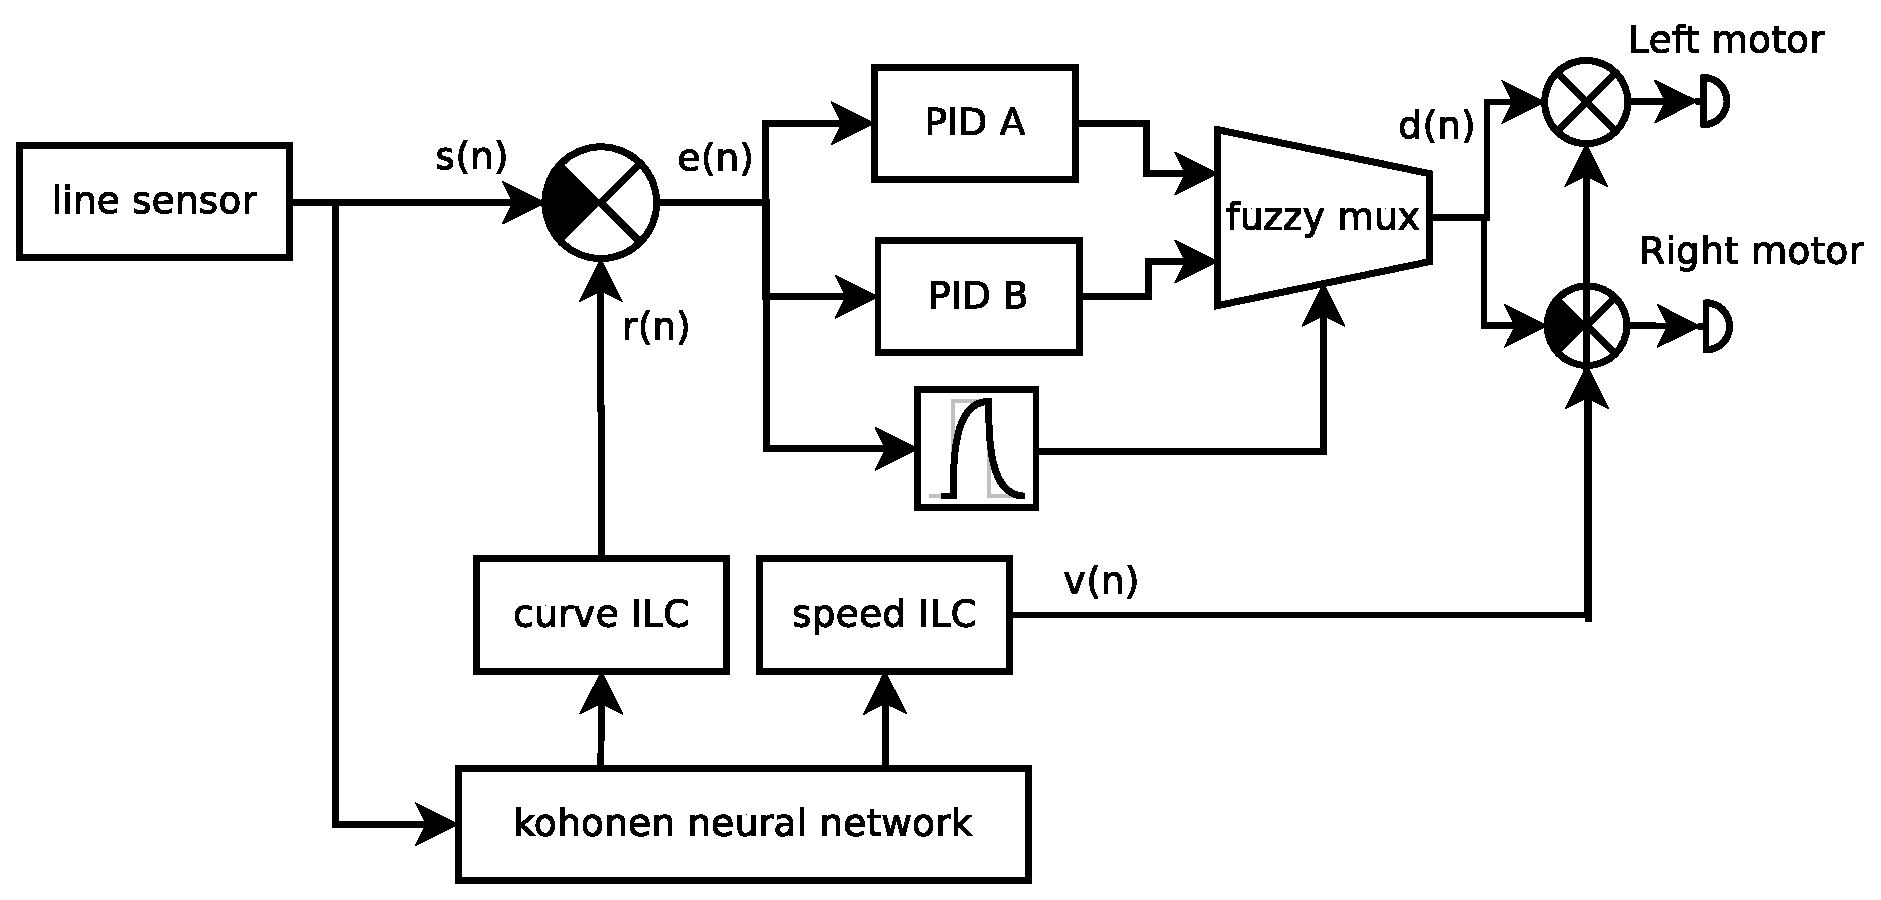
\includegraphics[width=1.0\textwidth]{block_diagram/robot_block.eps}
\end{center}
\end{minipage}
\end{center}
\end{figure}

\end{frame}

%-------------------------------------------------------------------------------------
\begin{frame}{\bf Kohonenova sieť}

\begin{figure}[ht]
\begin{center}
\begin{minipage}{0.6\linewidth}
\begin{center}
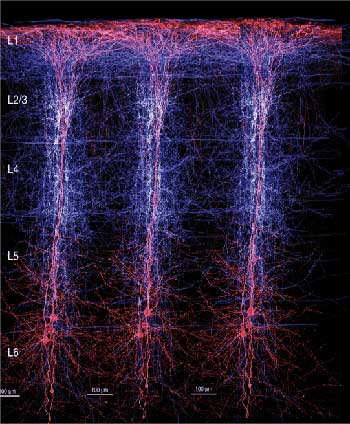
\includegraphics[width=1.0\textwidth]{images/cortical_column.jpg}
\end{center}
\end{minipage}
\end{center}
\end{figure}

\end{frame}

%-------------------------------------------------------------------------------------
\begin{frame}{\bf Kohonenova sieť}

\begin{figure}[ht]
\begin{center}
\begin{minipage}{0.6\linewidth}
\begin{center}
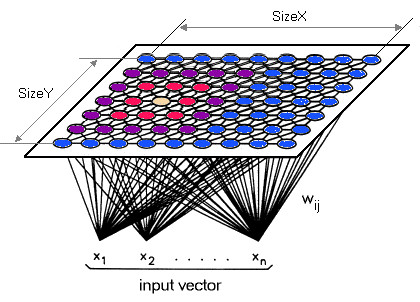
\includegraphics[width=1.0\textwidth]{images/kohonen.jpg}
\end{center}
\end{minipage}
\end{center}
\end{figure}

\end{frame}

%-------------------------------------------------------------------------------------
\begin{frame}{\bf Kohonenova sieť}

\begin{figure}[ht]
\begin{center}
\begin{minipage}{0.8\linewidth}
\begin{center}
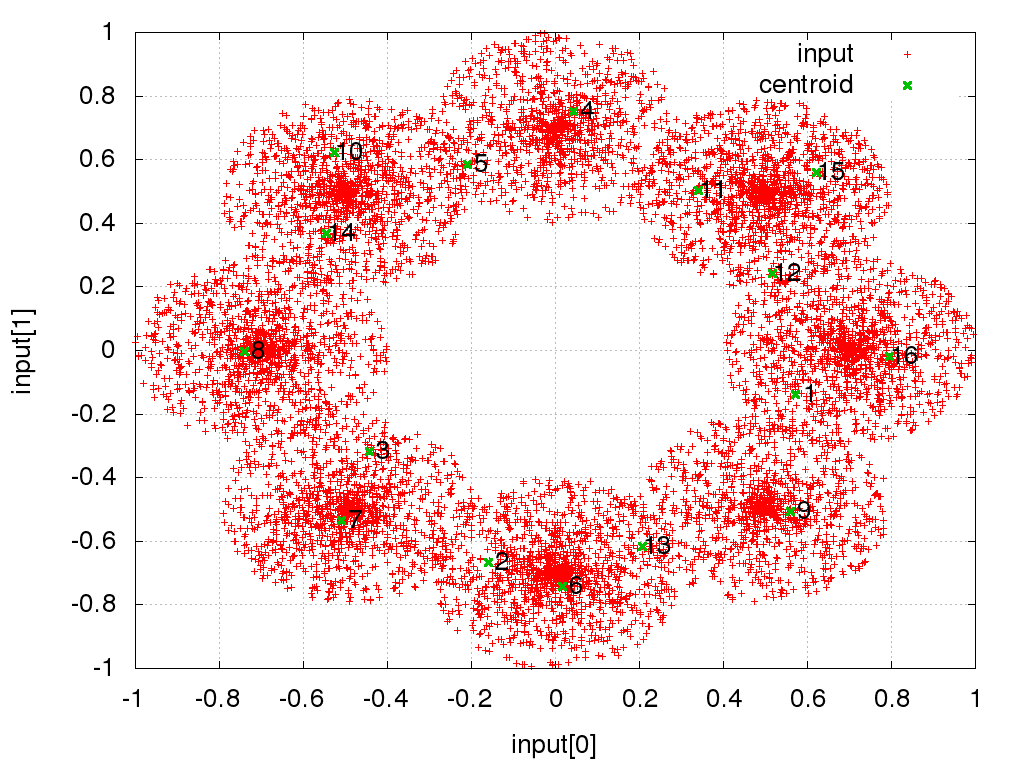
\includegraphics[width=1.0\textwidth]{kohonen_test/learing_result.png}
\end{center}
\end{minipage}
\end{center}
\end{figure}

\end{frame}


%-------------------------------------------------------------------------------------
\begin{frame}{\bf Kohonenova sieť - vo vnútri}

\begin{eqnarray}
\label{neuron_transfer}
y_j(n) &= \sum_{i = 0}^{M-1} {|s(n-i) - w_{ji}(n)|}, \\
w_q(n) &= \eta w_q(n-1) + (1 - \eta)S(n)
\end{eqnarray}

kde \\
$S(n)$ je predložený vzor (vektor so zložkami $S(n) = [s(n), s(n-1), ... , s(n-i)]$) ,\\
$w_j$ je vektor váh, pre každý neurón, \\
$w_q$ je vektor váh výťazného neurónu, \\
$\eta$ je rýchlosť učenia, obvykle $\eta \approx 0.99$.

\end{frame}

%-------------------------------------------------------------------------------------
\begin{frame}{\bf Výsledky klasifikácie zákrut}

\begin{figure}[ht]
\begin{center}
\begin{minipage}{0.8\linewidth}
\begin{center}
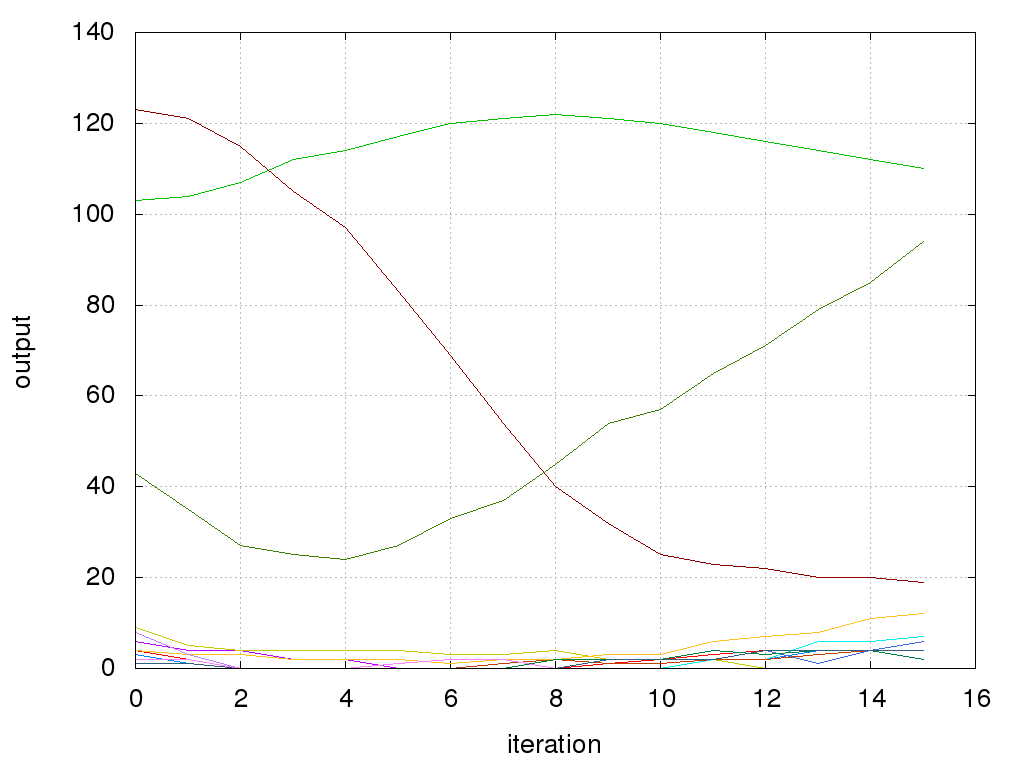
\includegraphics[width=1.0\textwidth]{prediction/predictor.png}
\end{center}
\end{minipage}
\end{center}
\end{figure}

\end{frame}

%-------------------------------------------------------------------------------------
\begin{frame}{\bf Ďalšie smerovanie}

\begin{enumerate}
	\item Pripojenie kamery
	\item Adaptívny regulátor
    \item Iný pohľad na \ref{eq_basic_robot}
	\item ... veľa testovania
\end{enumerate}

\end{frame}

%-------------------------------------------------------------------------------------
\begin{frame}{\bf Ďakujem za pozornosť}

\begin{figure}[ht]
\begin{center}
\begin{minipage}{0.4\linewidth}
\begin{center}
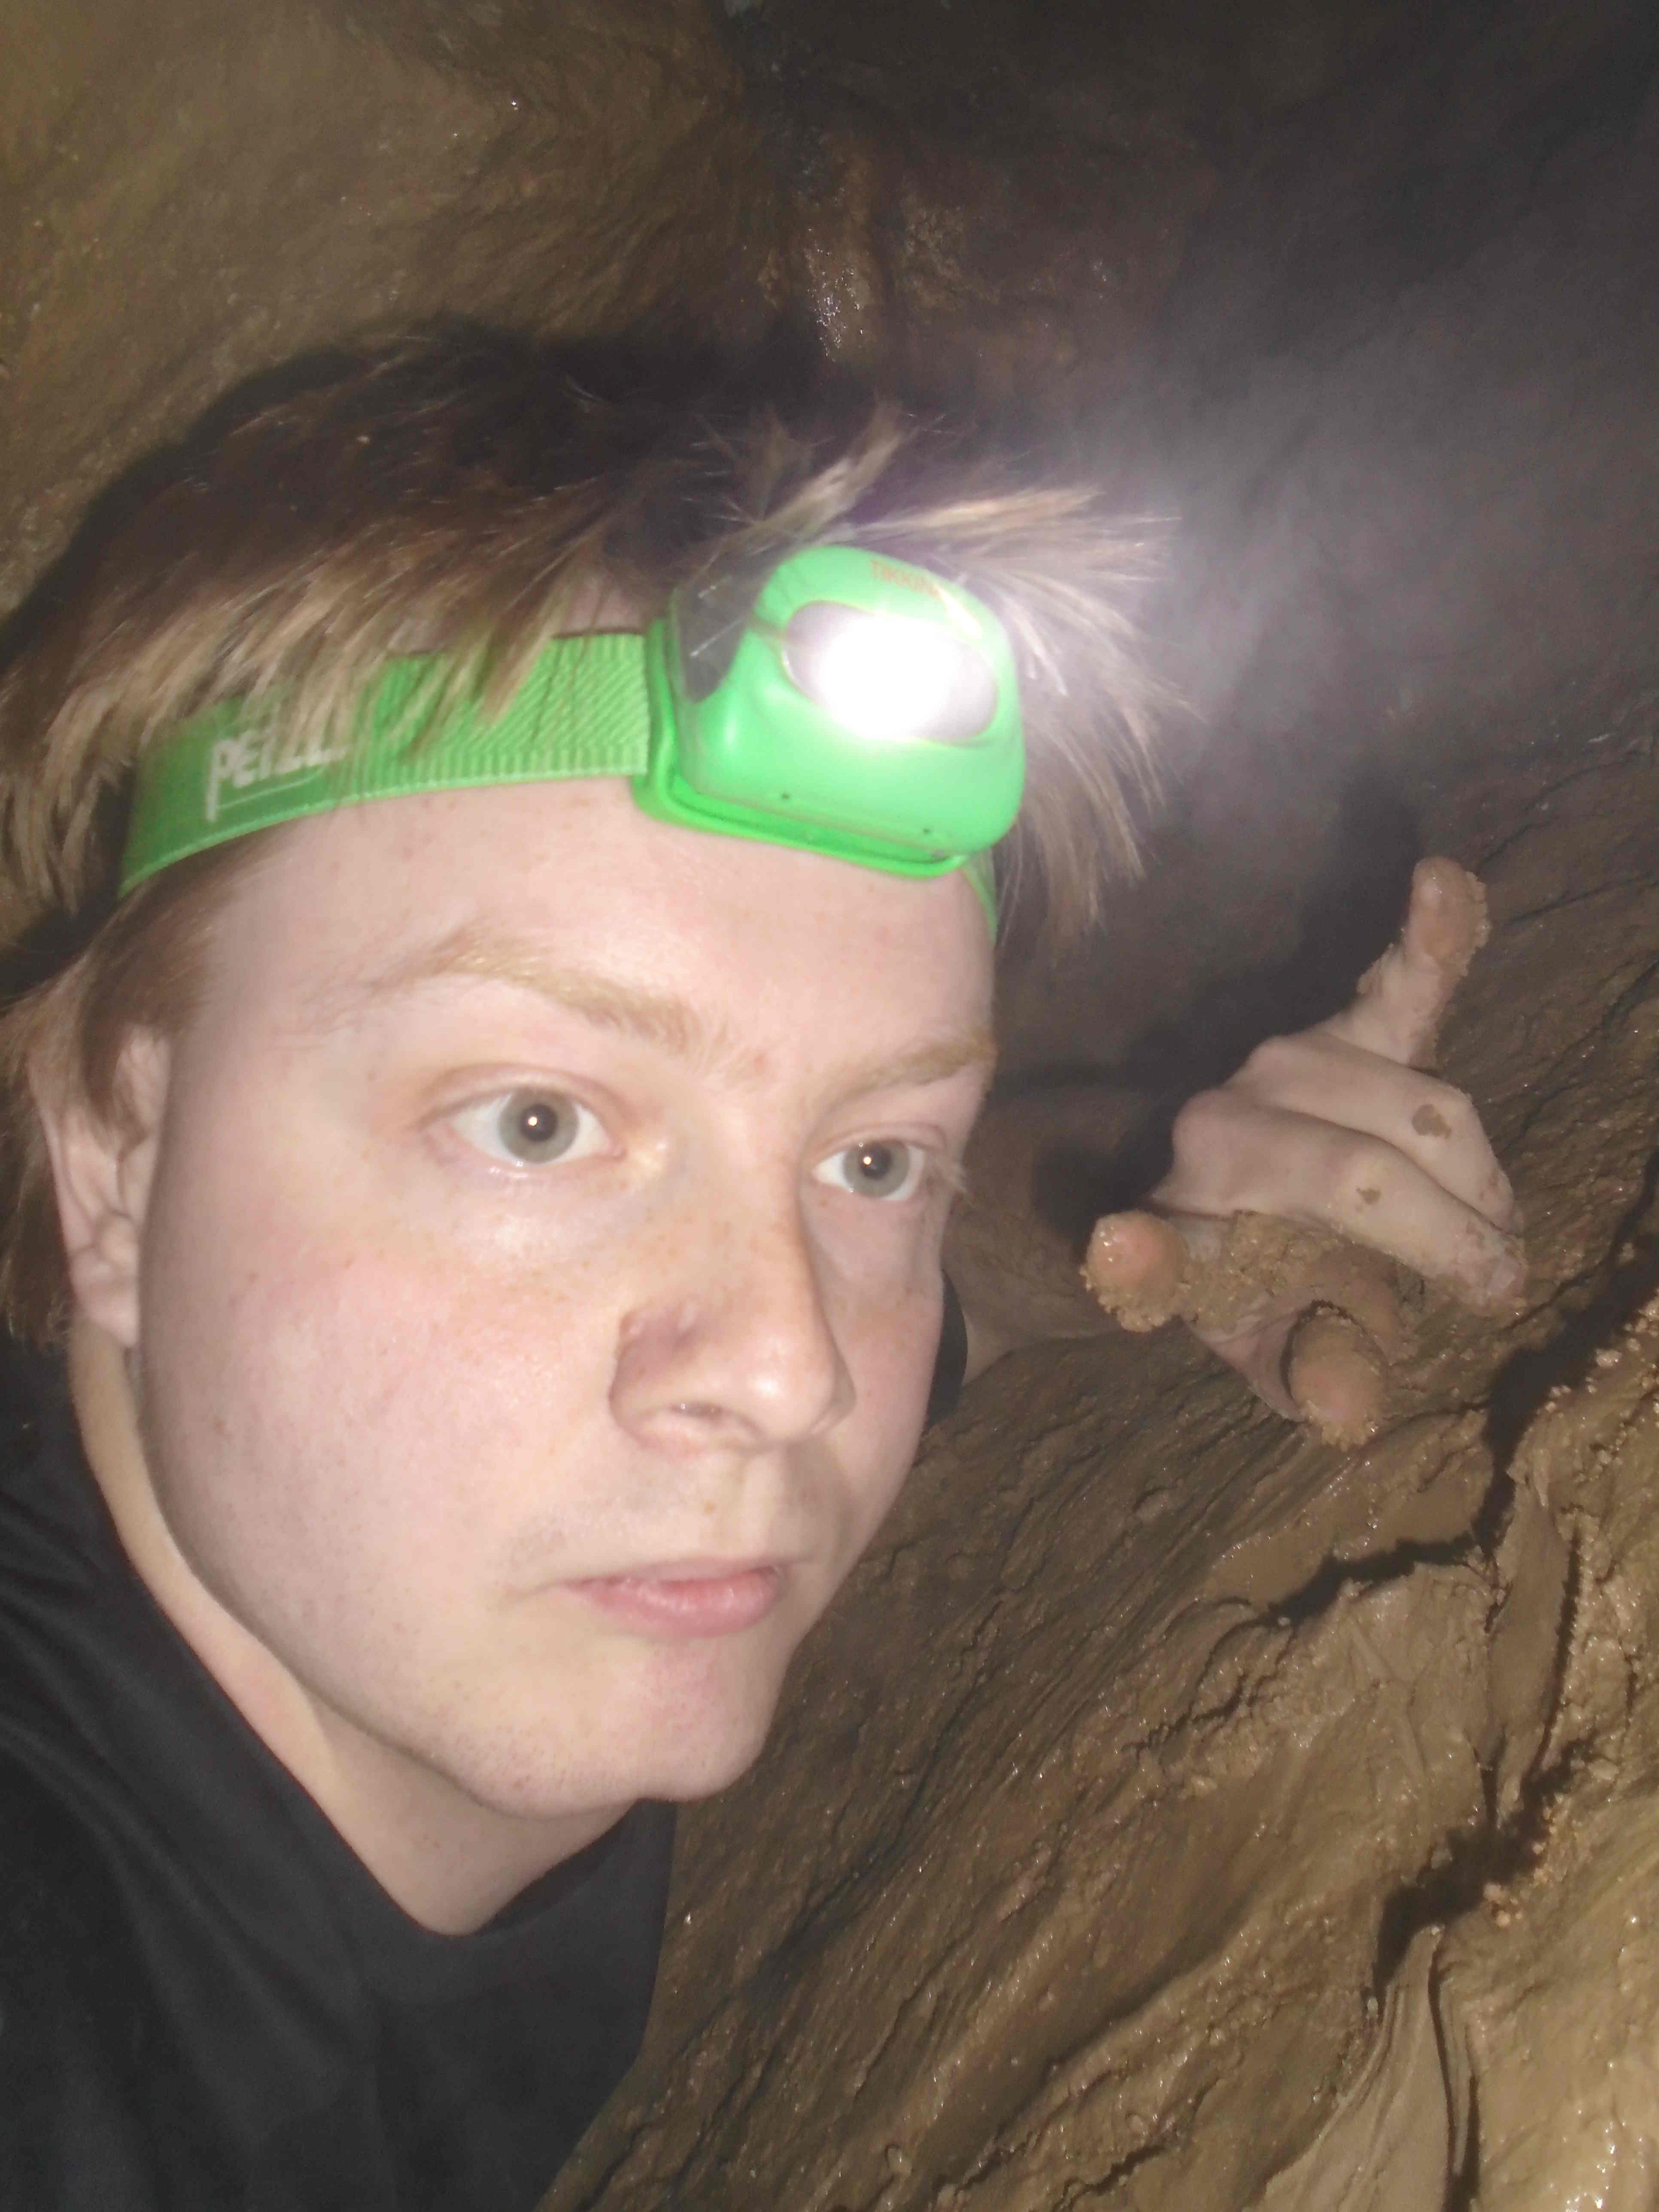
\includegraphics[width=1.0\textwidth]{images/cave.jpg}
\end{center}
\end{minipage}
\end{center}
\end{figure}


\centerline{michal.chovanec@yandex.ru}

\end{frame}

\end{document}
